% rubber : module pdftex
\documentclass{beamer}
%\usetheme{Berkeley}
%\usetheme{Antibes}
\usetheme{CambridgeUS}
\usecolortheme{dolphin}
\usepackage{varwidth}

\title%[SE390] % (optional, only for long titles)
{SE464 Project Deliverable 1 Presentation}
\subtitle{Group 17}
\author[SE2018] % (optional, for multiple authors)
{Software Engineering Class of 2018}
\institute[UW] % (optional)
{
  University of Waterloo
}
\date%[KPT 2004] % (optional)
{September 29, 2016}
\subject{Software Engineering}

%%% BEGIN PREAMBLE

\usepackage{geometry}
% \geometry{screen}
\title{Shots Fired}
\author{scmaier, d2lal, samiskin, wcakeize}

%%% BEGIN DOCUMENT
\begin{document}
\maketitle
\begin{frame}
\frametitle{Brief Project Description}
%  \begin{center}
%  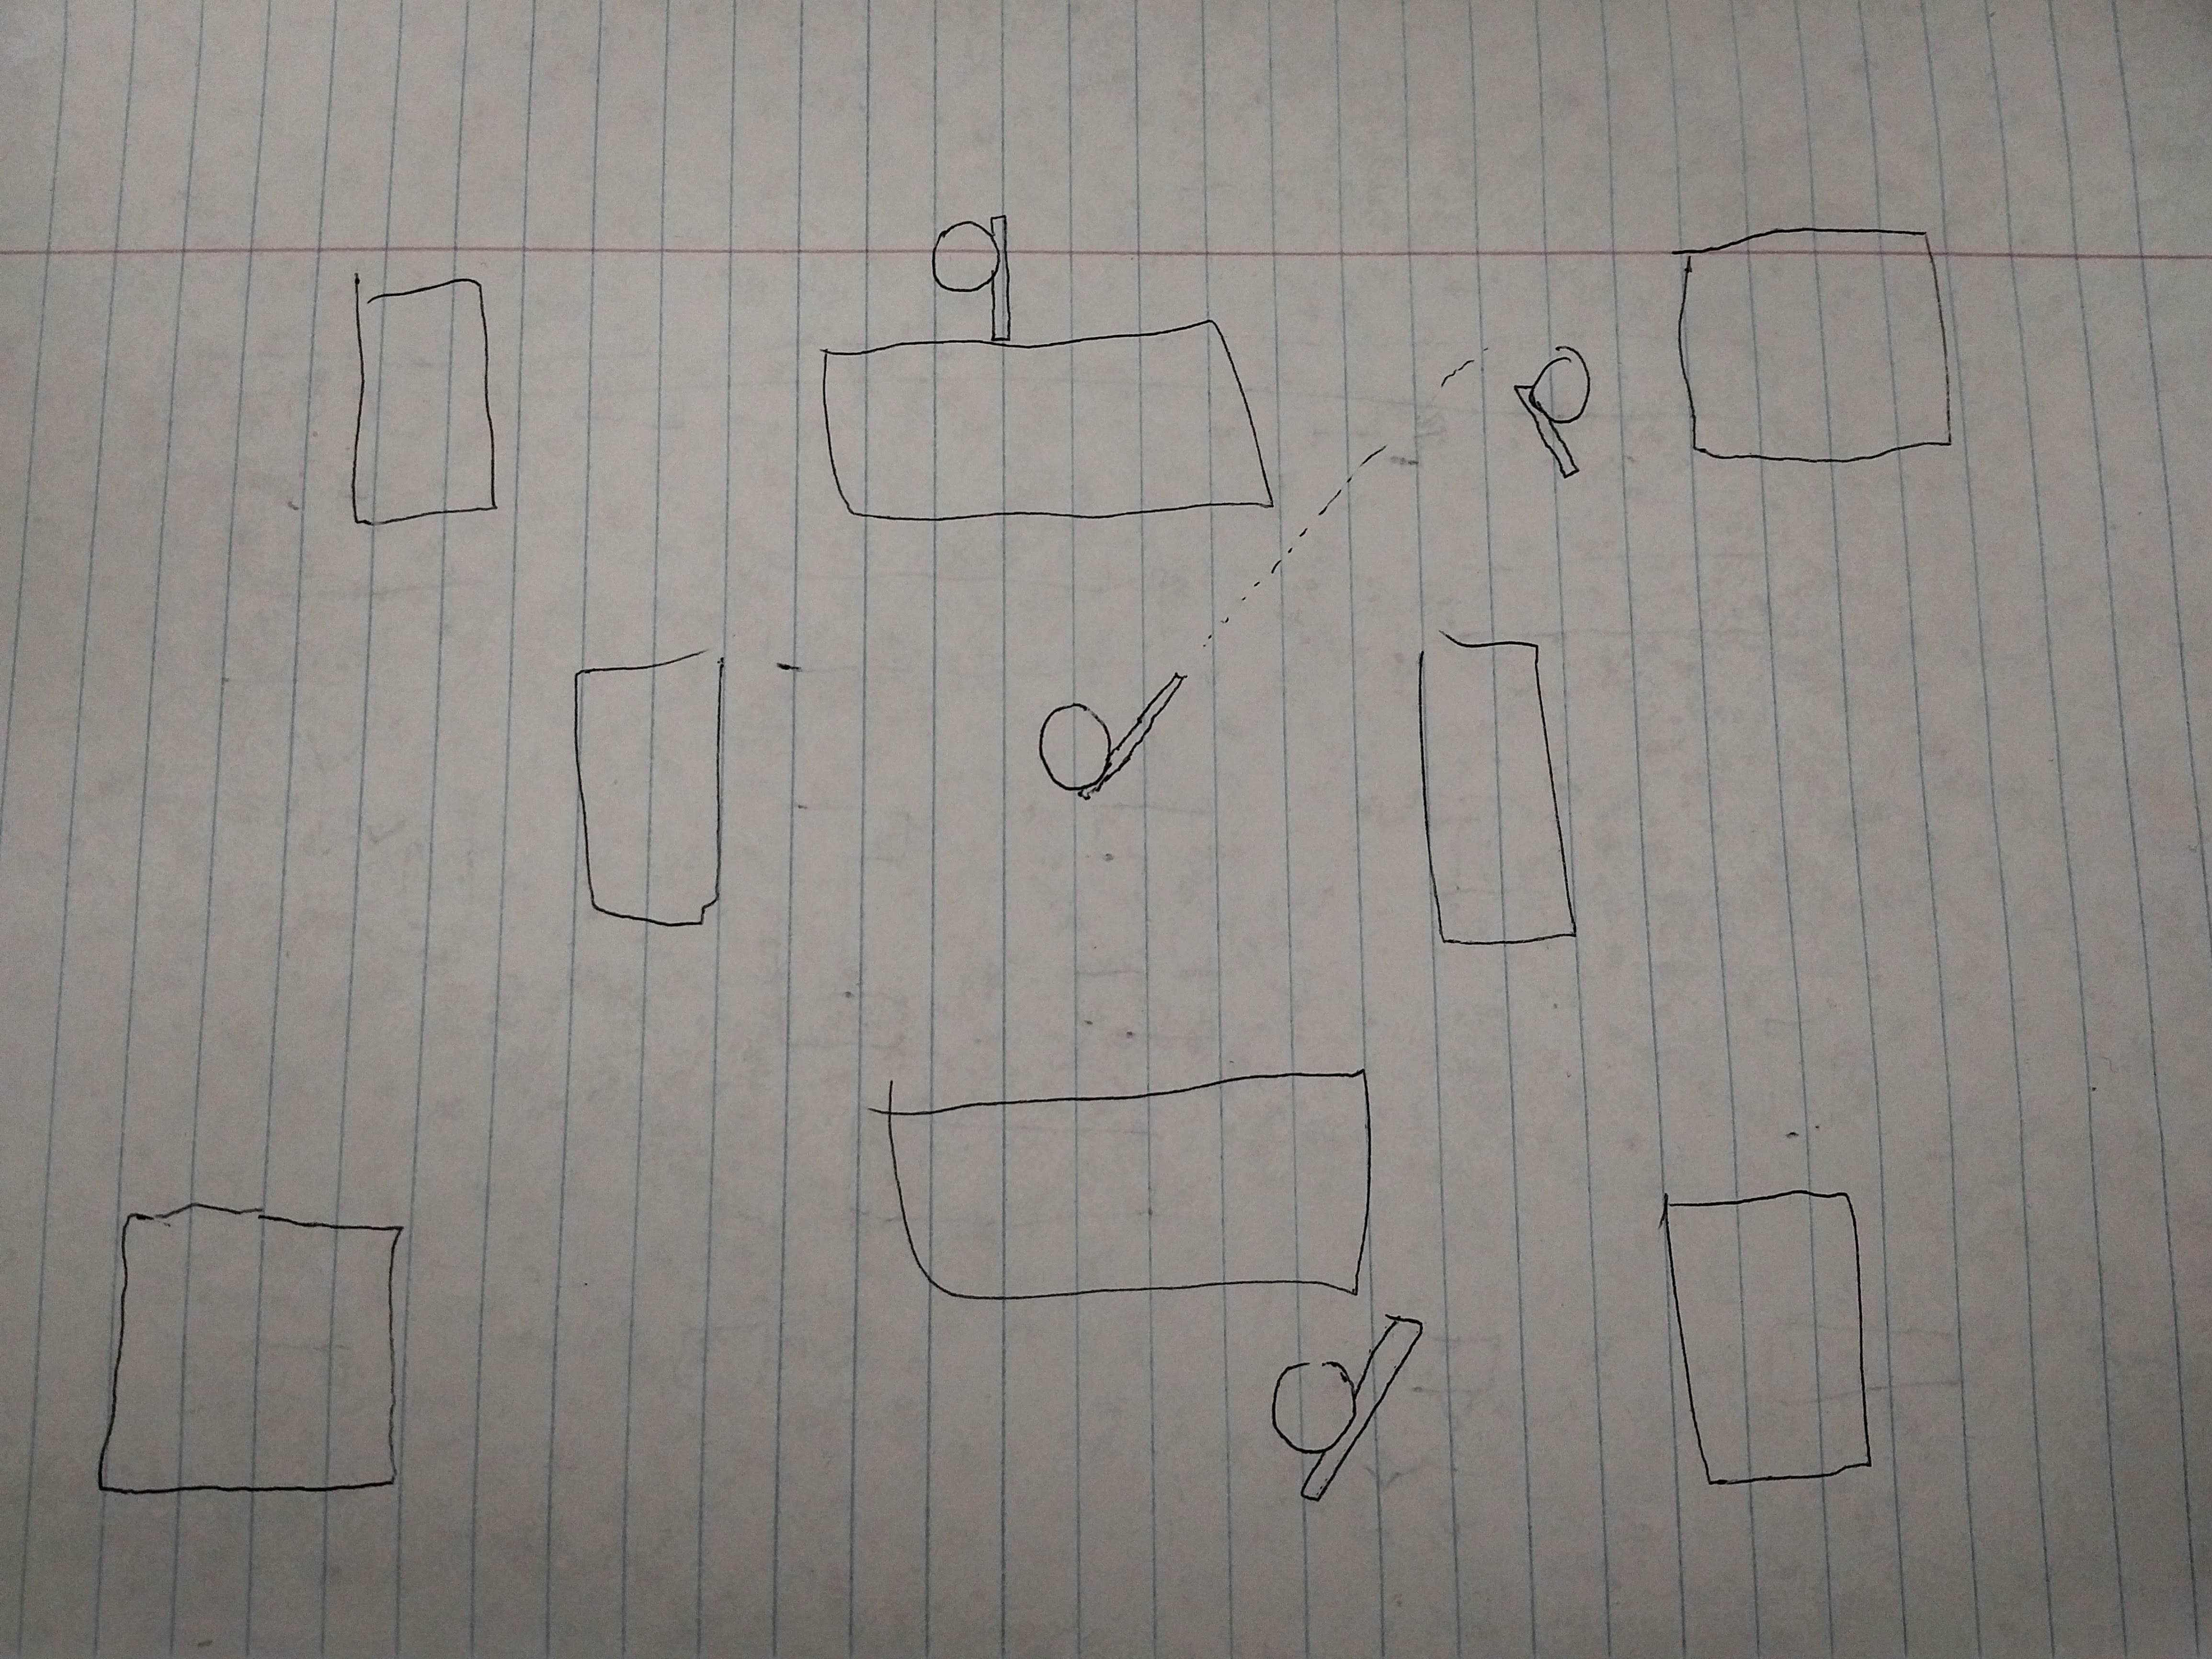
\includegraphics[scale=0.06]{images/mockup.jpg}
%  \end{center}
\begin{enumerate}
  \item Top-down arena style 2D online multiplayer shooting game
  \item Can easily join a game with friends (low barrier to entry)
  \item 2-4 player game played on separate machines connected online
  \item When a player loses all their health they are out
  \item Last person standing wins!
\end{enumerate}
\end{frame}

\begin{frame}
\frametitle{Game Screen Capture}
\centering
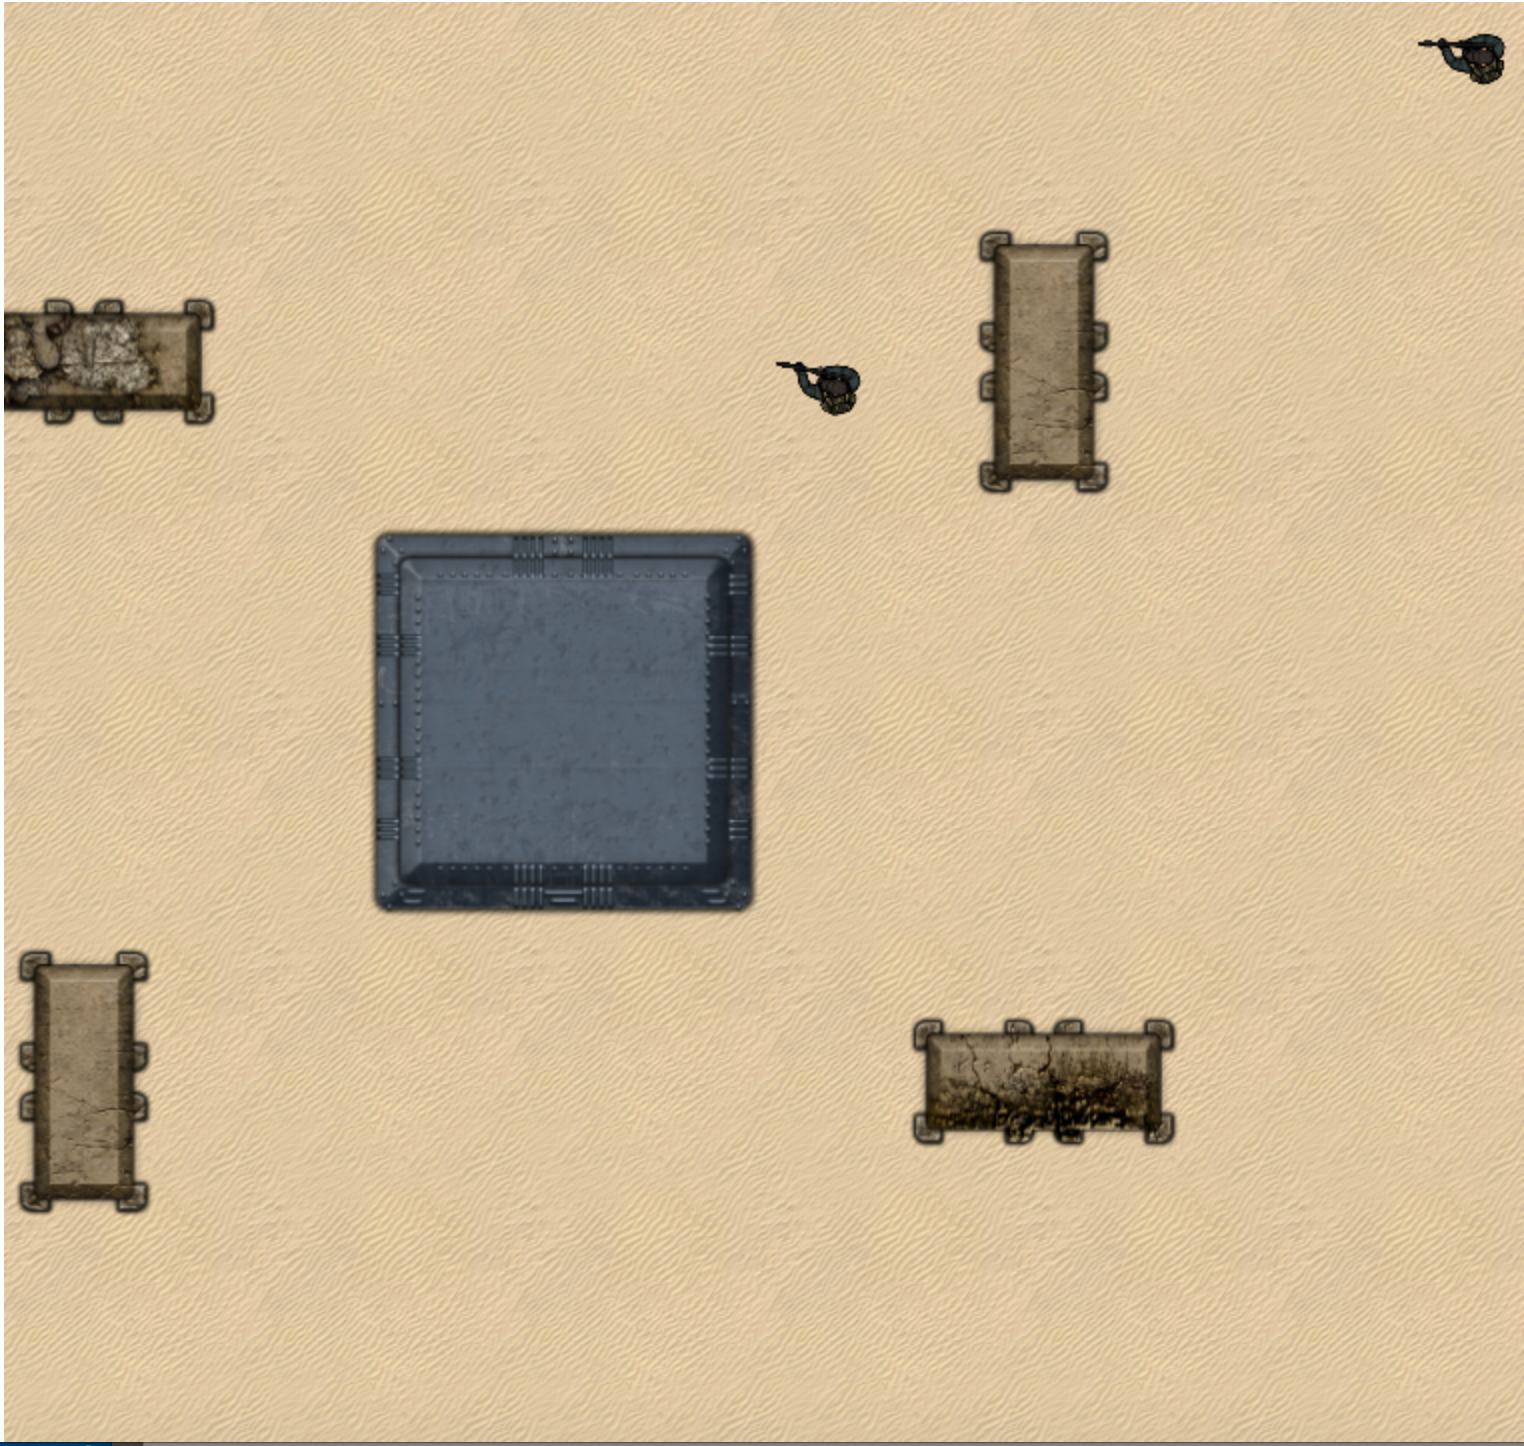
\includegraphics[scale=0.3]{images/gamescreenshot.png}
\end{frame}

\begin{frame}
\frametitle{Gameplay}
\begin{enumerate}
  \item Each player has x amount of health
  \item Move with WASD
  \item Move mouse to aim.
  \item Click to fire.
\end{enumerate}
\end{frame}

%\begin{frame}
%\frametitle{End of Game}
%\begin{enumerate}
%  \item If the user won, they are presented with a winners screen
 % \item If the user lost, they are presented with a game over screen
%\end{enumerate}
%\end{frame}

\begin{frame}
\frametitle{Design Challenges}
\begin{enumerate}
  \item Creating a game with character interactions, animations, controls, physics, online connections
  \item Synchronizing differences between client and server game states
  \item Running and managing multiple game servers simultaneously
  \item Ensuring easily extendable game object interaction. 
\end{enumerate}
\end{frame}

\begin{frame}
\frametitle{Handling Game Operations}
\begin{enumerate}
  \item Various operations were split into stages, each modifying the game state
    and passing it to the next stage, resembles pipe and filter
    \begin{enumerate}
      \item Apply game inputs
      \item Handle any game object deletions
      \item Update individual entities
      \item Resolve interactions between entities
    \end{enumerate}
  \item Interactions between entities handled using events
  \item Attempted a more functional approach, however mutability was still
    allowed for performance reasons, as updates are made at 60 frames per
    second.
\end{enumerate}
\end{frame}

\begin{frame}
\frametitle{Client Synchronization}
\begin{enumerate}
  \item Clients forward \textbf{only their inputs} to the server
  \item Game continues to be simulated on the clients
  \item Server collects inputs from all clients
  \item Server applies inputs and updates
  \item Server forwards the entire state of the game to clients (the game state
    acts as a blackboard)
  \item Clients re-sync on receiving the server copy
\end{enumerate}
\end{frame}

\begin{frame}
\frametitle{Mitigating Latency Effects}
\begin{enumerate}
  \item The game state received by the server may be significantly delayed
  \item The server copy is simulated up to the current time on the client
  \item Inputs from the client which occured after the time of the server update
    are reapplied

\end{enumerate}
  \centering
  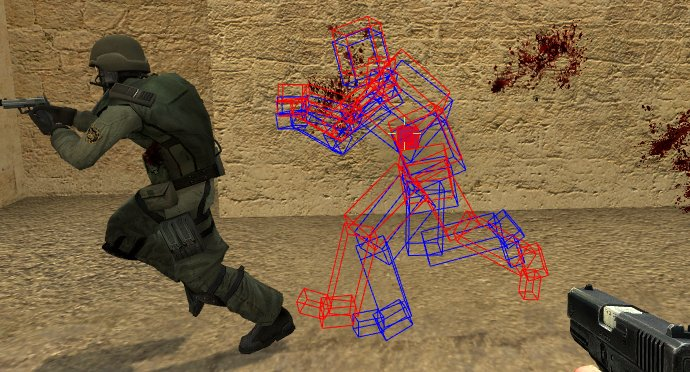
\includegraphics[scale=0.25]{images/csgo-lag-compensation.png}
\end{frame}

\begin{frame}
  \frametitle{Node.js Concurrency}
\begin{enumerate}
  \item Efforts were made to improve performance through concurrency, using
    multiple cores
  \item Problems due to JavaScript being single-threaded by design and Node.js having
    poor multi-process support
  \item Issues also arise with deployment due to only one port being allowed
\end{enumerate}
\end{frame}
%\begin{frame}
%\frametitle{Requirements}
%\begin{enumerate}
%  \item Top-down arena style 2D shooting game
%  \item 2-4 player game played on separate machines connected online
%  \item Characters are controlled with Keyboard and Mouse
 % \item Can easily join a game with friends (low barrier to entry)
%\end{enumerate}
%\end{frame}

\begin{frame}
\frametitle{Overall Architecture}
\centering
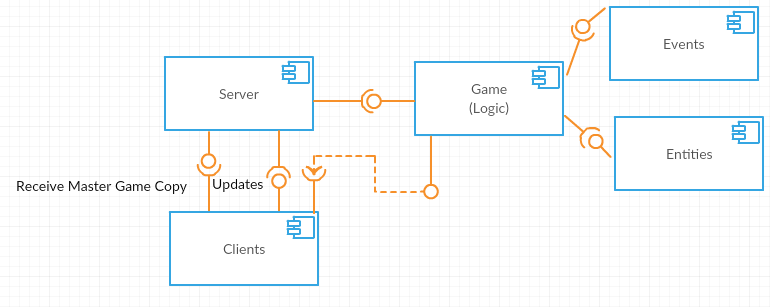
\includegraphics[scale=0.4]{images/overall_architecture.png}
\end{frame}

\begin{frame}
\frametitle{Server Architecture}
\centering
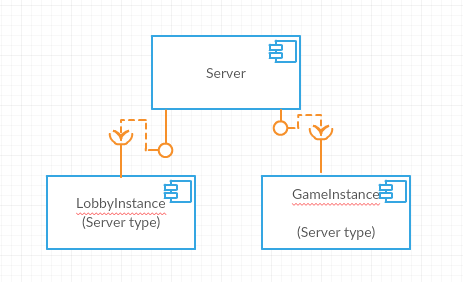
\includegraphics[scale=0.7]{images/ServerArchitecture.png}
\end{frame}

\begin{frame}
\frametitle{Client Architecture}
\centering
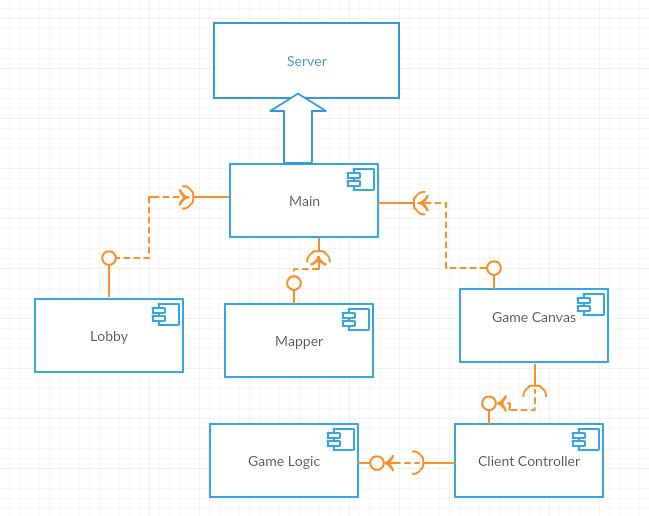
\includegraphics[scale=0.4]{images/ClientArchitecture.png}
\end{frame}


\end{document}

